	\section{Exkurs: Emergenz der Entropie}
	
	\begin{center}
		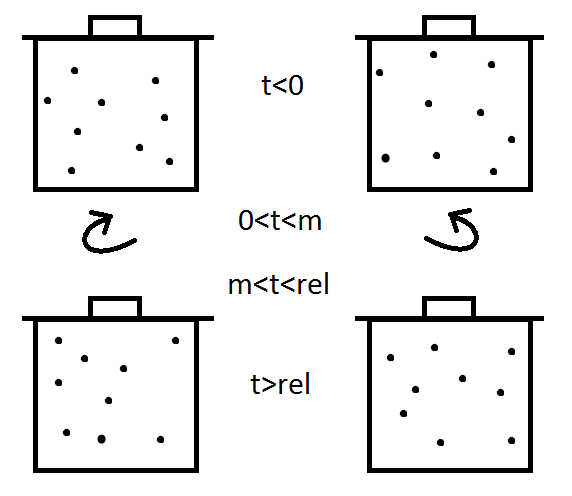
\includegraphics[width=0.6\textwidth]{Abb/Emergenz.png}
	\end{center}%
	Man stelle sich zwei mit Gas gefüllte Behälter in zwei verschiedenen Laboratorien vor. Beide besitzen -innerhalb einer gewissen Fehler\-toleranz- die gleichen charakteristischen Zustandsgrößen und lassen sich anhand dieser zum Zeitpunkt $t<0$ nicht unterscheiden. Im Zeitintervall $0<t<m$ werden die beiden Behälter nun in unterschiedliche Richtungen gerührt und sind im folgendem $m>t>rel$ voneinander unterscheidbar. Nach einer gewissen Relaxationszeit $rel$ befinden sich die beiden Gase wieder im Gleichgewicht und sind makroskopisch nicht mehr voneinander zu unterscheiden. Die makroskopische Beschreibung hat das Rühren "vergessen". 

	
\chapter{Grundlegende Konzepte der Statistik und der Wahrscheinlichkeitstheorie}

	\paragraph{klassische Mechanik:}
		Mittelwert, Varianz, Verteilungsfunktionen, Korrelationen ect.
	\paragraph{QM:}
		analoge Bildungen.
		
	\section{Klassische Statistik}
	
	\begin{figure}[H]
		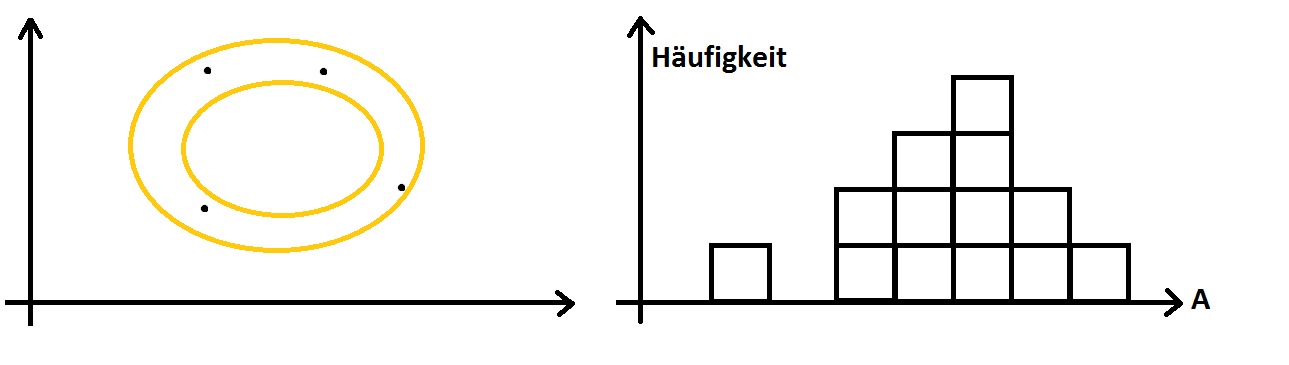
\includegraphics[width=0.9\textwidth]{Abb/abb21.png}
		\caption{Links: bildliche Darstellung der Menge aller Ensemble im 6N-Dimensionelen Raum mit Achsen $p$ und $x$.\\ Rechts: Histogramm (oft $\frac{\text{Häufigkeit}}{\text{Anzahl}}$, so dass dieses normiert ist.)}
		\label{HTT}
	\end{figure}
		
	Aus der Abb. \ref{HTT} folgt intuitiv die Definition des Mittels. Um dieses zu erhalten Summiert man alle Werte $A(p^{(j)},x^{(j)})$ des betrachteten Ensembles $\{p^{(j)},x^{[j]}\}, j=1,...,J $ und Teilt durch die Anzahl der Elemente des selbigen.
	\begin{align*}
		\langle A \rangle = \frac{1}{J} \sum_{j=1}^{J} A(p^{(j)},x^{(j)}) \\
	\end{align*}
	
	\noindent Durch den Übergang zu beliebig genauen Messgenauigkeiten, wird die diskrete Verteilung in Abb. \ref{HTT} zu einer kontinuierlichen Kurve. (Übergang zum Kontinuumslimes.)
	
	\begin{figure}[H]
		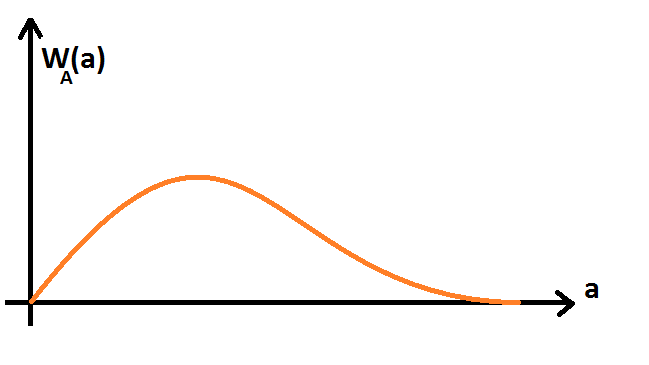
\includegraphics[width=0.9\textwidth]{Abb/abb22.png}
		\caption{Übergang zum "Kontinuumslimes" mit Wahrscheinlichkeit $W_A(a)$.}
	\end{figure}
	\noindent Wie oben ist auch diese Kurve normiert. Die Häufigkeit wird ersetzt durch $W_A(a)$, welche die Wahrscheinlichkeit angibt, für ein gegebenes Ensemble, eine Messgröße $A$ mit dem Wert $a$ zu Messen. 	
	\newline \newline
	Im Folgenden sollen nun noch kurz einige wichtige Begrifflichkeiten aus der Statistik definiert werden.
	
	\paragraph{Varianz:}
	\[\langle [A - \langle A \rangle]^2 \rangle  = \langle A^2 \rangle - \langle A \rangle^2 \]
	\paragraph{Weitere Momente:}\footnote{Definition und mehr auch im Bronstein "Taschenbuch der Mathematik"}
	\[ \langle A^k \rangle = \frac{1}{J} \sum_{j=1}^{J}(A(p^{(j)},x^{(j)}))^k \]
	\paragraph{Phasenraumdichte:}\footnote{$ \delta(p-p^{(j)}) = \delta(p_{1x}-p_{1x}^{(j)}) \cdot \delta(p_{1y}-p_{1y}^{(j)})\cdot ... \cdot \delta(p_{Nz}-p_{Nz}^{(j)})$.}
	\[ \rho (p,x) = \frac{1}{J} \sum_{j=1}^{J} \delta(p-p^{(j)}) \delta(x-x^{(j)}) \]
	
	\noindent Mithilfe der Phasenraumdichte lässt sich jetzt der Mittelwert auch mithilfe eines Integrals beschreiben: 
	\[ \langle A \rangle \int dp^{3N} dx^{3N} \rho (p,x) A(p,x)\]
	
	\subsection{Motivation für die Einführung der Phasenraumdichte:}
	Zum einen erlaubt die Einführung durch Produktbildung die Trennung der Eigenschaften von Beobachtungsgrößen und Ensemble, zum anderen ist dies die mathematische Umsetzung des Übergangs vom mikroskopischen zum makroskopischen (Coarse-Graining). 
	
	\subsection{Generische Eigenschaften von $\rhopx$}

\begin{enumerate}
	\item $\rhopx$ ist reell\\
	\item $\rhopx \geq 0$\\
	\item $\dpdx \rhopx = 1$
\end{enumerate}
\paragraph{Bemerkung:} Wir können $\rhopx$ als Wahrscheinlichkeitsdichte
interpretieren.
\begin{align*}
	&\erw{A} = \dpdx \rhopx A(p,x)\\
	&\wkeit{A}{a} = \erw{\deltaa} = \dpdx \rhopx \delta ( a - A(p,x) )
\end{align*}

	\subsection{Korrelation}

\begin{center}
	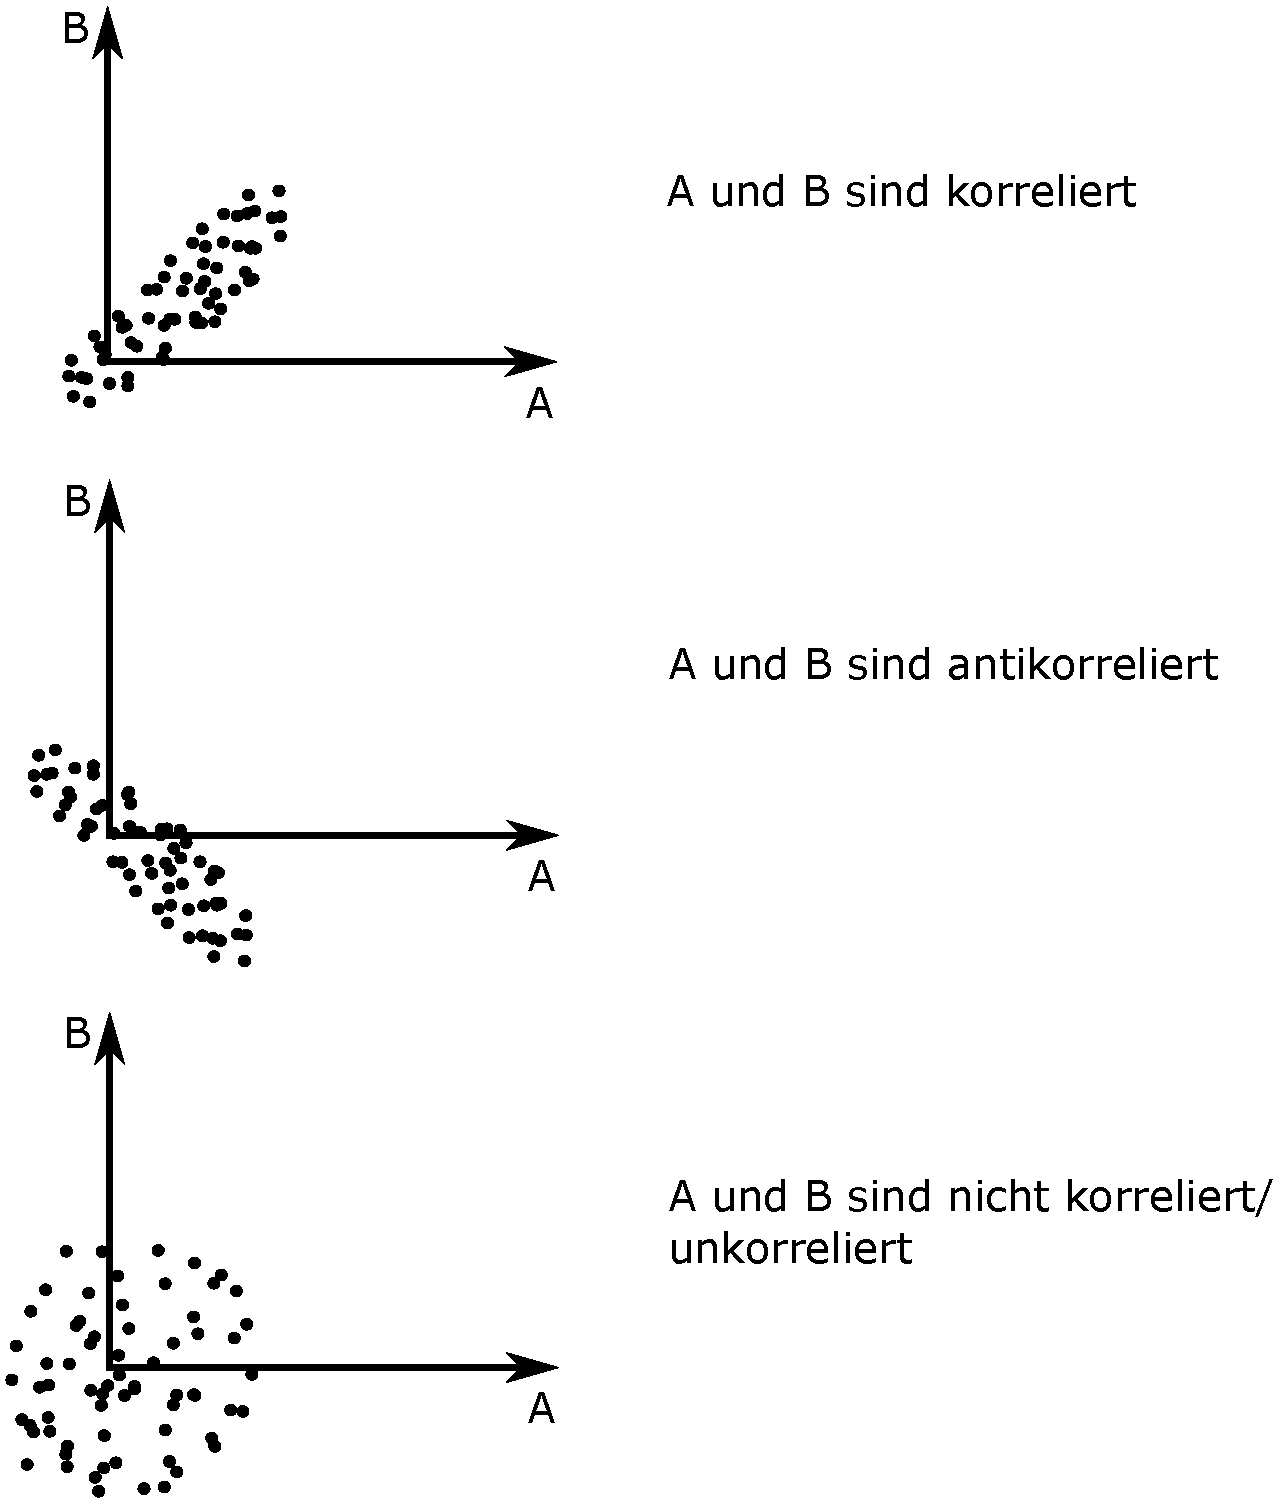
\includegraphics[width=0.8\textwidth]{Abb/korrelation.pdf}
\end{center}

\paragraph{Bemerkung:} Neben Mittelwerten von Observablen sind auch deren
Korrelationen ein wichtiges Charakteristikum eines physikalischen Zustands.\\
$\rightarrow$ Fluktuations-Dissipations-Theorem

\begin{align*}
	K_{AB} &= \erw{\var{A} \var{B}}\\
		   &= \frac{1}{J} \sum_{j=1}^{J} \big( A^{(j)} - \erw{A} \big) \big( 
		      B^{(j)} - \erw{B} \big)\\
		   & A^{(j)} = A(p^{(j)}, x^{(j)})
\end{align*}

\paragraph{Paarwahrscheinlichkeit:} 
\begin{align*}
	\wkeit{AB}{a,b} &= \erw{ \deltaa \deltab }\\
				   &= \dpdx \rhopx \deltaa \deltab
\end{align*}

\paragraph{Eigenschaften:}
\begin{align*}
	1.\; &\wkeit{A}{a} = \int db \, \wkeit{AB}{a,b}\\
	     &\wkeit{B}{b} = \int da \, \wkeit{AB}{a,b}\\
	2.\; &K_{AB} = \int da \, db \, ( a - \erw{A} ) (b - \erw{B} ) \, 
	     \wkeit{AB}{a,b}
\end{align*}

\paragraph{Definition: statistisch unabhängig}
\[
	\wkeit{AB}{a,b} = \wkeit{A}{a} \cdot \wkeit{B}{b}
\]
Beispiel für statistisch unabhängige Größen, sind die einzelnen Würfe beim Münzwurf.

\subparagraph{Anwendung:}
Betrachten wir zwei komplett getrennte Gase und wollen deren Eigenschaften
untersuchen, so gilt:
\begin{align*}
	&\rhopx = \rho (p_{1}, x_{1}) \rho (p_{2}, x_{2})\\
	&p=(p_{1},p_{2}) \quad x = (x_{1}, x_{2})
\end{align*}

	\section{Quantenstatistik}
	\subsection{Quanten-Mittelwerte}

\subparagraph{Beispiel:} Fock-Raum als Analogon zum klassischen Phasenraum für $N$
Fermionen\\

Vielteilchenwellenfunktionen von Fermionen sind vollständig antisymmetrisiert
("`Slater-Determinante"'), Bosonen haben dagegen eine vollständig symmetrisierte 
Wellenfunktion

\[
    \hat{H} = \sum_{i=1}^{N} \left( - \frac{1}{2m} \frac{d^{2}}{d\ri} + V_{ex}
               (\ri) \right) + \frac12 \sum_{i \neq j}{N} v(\ri - \rj)
\]

z.B.: $v(\vec{r}) = \frac{R^{2}}{|\vec{r}|}$

\paragraph{Zeitentwicklung:}
\[
    i \partial_{r} \psirn = \hat{H} \psirn
\]

Zum Phasenraum für Fermionen:
Dieser Phasenraum wird aufgespannt durch alle möglichen Slaterdeterminanten, die man
bilden kann: 
\[{}
    \ket{SD_{1}} \ket{SD_{2}} \dots{}
\]
Eine Wellenfunktion wird in diesem Raum durch einen Punkt dargestellt.
Sei nun $\ket{j}$ eine Menge/Ensemble von Mikrozuständen der QM (Wellenfunktionen)
$j = 1,\dots, J$. Die Zustände $\ket{j}$ seien kompatibel mit den experimentellen 
Randbedingungen, z.B. Teilchenzahl, Gesamtenergieinhalt,...\\
Für einen Teilchenzustand $\ket{j}$ ist sein Beitrag zum Ensemble:
\begin{align*}
    &A^{(j)} := \braket{j | \hat{A} | j}\\
    &\erw{\A} := \frac{1}{J} \sum_{j=1}^{J} \braket{j| \A | j} \quad 
    \text{(Mittelwert)}
\end{align*}

    \subsection{Dichteoperator}

\paragraph{Vollständigkeit:} $\mathds{1} = \sum_{\mu} \ket{\mu} \bra{\mu}$, $\mu$ 
ist ein Basisvektor im Vektorraum

\begin{align*}
    \erw{\A}&= \frac{1}{J} \sum_{j=1}^{J} \braket{j | A | j} = \frac{1}{J} 
               \sum_{j} \sum_{\mu} \braket{j|\mu}\braket{\mu|\A|j}\\
    \quad   &= \frac{1}{J} \sum_{j} \sum_{\mu} \braket{\mu|\A|j}\braket{j|\mu}\\
    \dop    &= \jnorm \sum_{j} \ket{j}\bra{j} \quad 
              \text{Dichteoperator der QS}\\
    \erw{\A}&= \sum_{\mu} \braket{\mu| \A \dop |\mu} = \tr (\A \dop)
\end{align*}

\paragraph{Anwendung im mikroskopischen System:}
\[{}
    \dop = \frac12 \left( \ket{\uparrow} \bra{\downarrow} + \ket{\leftarrow} 
                           \bra{\leftarrow} \right){}
\]
{}
Die Zusammensetzung der Ensembles soll in der Übung behandelt werden.

\paragraph{Eigenschaften von $\dop$:}
\begin{enumerate}
    \item Hermitizität: $\braket{\mu|\dop|\nu} = \braket{\nu|\dop|\mu}^{*}$\\
    \item Positivität: $\braket{\dots|\dop|\dots} \geq 0$ für jedes 
          $\ket{\dots}$\\
    \item Normierung: $\sum_{\mu} \braket{\mu|\dop|\mu} = \tr \dop = 1$
\end{enumerate}

